\documentclass[paper=a4, fontsize=11pt, twocolumn]{scrartcl}

%%% LANGUAGE SETTINGS %%%
\usepackage[ngerman]{babel}							% German language/hyphenation
\usepackage[german]{babelbib}

\usepackage[utf8]{inputenc}
\usepackage[left=3cm,right=2cm,top=2cm,bottom=2cm,includeheadfoot]{geometry}
\usepackage[protrusion=true,expansion=true]{microtype}				% Better typography
\usepackage{amsmath,amsfonts,amsthm}							% Math packages

\usepackage[hang, small,labelfont=bf,up,textfont=it,up]{caption}			% Custom captions under/above floats

\usepackage[pdftex]{graphicx}										% Enable pdflatex

\usepackage{booktabs}											% Nicer tables
\usepackage{tabularx}

\usepackage[colorlinks=false,breaklinks=true,backref=none]{hyperref}
\usepackage{url}

\usepackage{listings}

\usepackage{abstract}
\usepackage{blindtext}

\bibliographystyle{acm}

%%% Advanced verbatim environment
\usepackage{verbatim}
\usepackage{fancyvrb}
\DefineShortVerb{\|}											% delimiter to display inline verbatim text

%%% Custom sectioning (sectsty package)
\usepackage{sectsty}											% Custom sectioning (see below)
\allsectionsfont{%												% Change font of al section commands
	\usefont{OT1}{bch}{b}{n}%									% bch-b-n: CharterBT-Bold font
}

\sectionfont{													% Change font of \section command
	\usefont{OT1}{bch}{b}{n}										% bch-b-n: CharterBT-Bold font
	\sectionrule{0pt}{0pt}{-5pt}{0.8pt}								% Horizontal rule below section
}

%%% Custom headers/footers (fancyhdr package)
\usepackage{fancyhdr}
\pagestyle{fancyplain}
\fancyhead{}													% No page header
\fancyfoot[C]{\thepage}											% Pagenumbering at center of footer
\renewcommand{\headrulewidth}{0pt}								% Remove header underlines
\renewcommand{\footrulewidth}{0pt}								% Remove footer underlines
\setlength{\headheight}{13.6pt}

%%% Equation and float numbering
\numberwithin{equation}{section}									% Equationnumbering: section.eq#
\numberwithin{figure}{section}										% Figurenumbering: section.fig#
\numberwithin{table}{section}										% Tablenumbering: section.tab#



%%% Title
\title{ \vspace{-1in} 	\usefont{OT1}{bch}{b}{n}
		\huge \strut  Proseminar: Peer-To-Peer Overlay Network Systems\strut \\
		\Large \bfseries \strut Fasttrack \strut
}

\author{ 					\usefont{OT1}{bch}{m}{n}
        Martin Görick\\		\usefont{OT1}{bch}{m}{n}
        Freie Universität Berlin\\	\usefont{OT1}{bch}{m}{n}
        \texttt{goerickm@zedat.fu-berlin.de}
}

%%% Begin document
\begin{document}
\twocolumn[
\begin{@twocolumnfalse}
\maketitle
\begin{abstract}
FastTrack ist ein Peer-To-Peer Overlay Netzwerk und ist dafür entwickelt worden Daten auszutauschen. 
In dieser Ausarbeitung werden die Funktionsweise des Protokoll beschrieben, wie es aufgebaut ist, welche Nachrichten verschickt werden oder wie Daten gesucht werden.
\vspace{4em}
\end{abstract}
\end{@twocolumnfalse}
]

\section{Einleitung}
FastTrack ist ein proprietäres Protokoll für ein Peer-To-Peer Overlay Netzwerk, welches von Niklas Zennstrom und Janus Friis entwickelt wurde, um Daten auszutauschen. \cite{liang2006fasttrack}
Es ist ein Projekt von den Unternehmen Sharman Networks \cite{sharmanN}, AltNet \cite{fastTrack} und Joltid \cite{joltid}.
In dieser Ausarbeitung geht es darum das Protokoll zu beschreiben.
Dabei wird zuerst Allgemeine Information in \ref{sec:allgInfo} dargestellt.
Dort geht es um die Aufbau des Netzwerkes und den Aufbau des Windows Programms.
Danach im Abschnitt \ref{sec:funkw} die Funktionsweise des Protokolls, wie das Betreten, das Suchen im Netzwerk und den Nachrichten von FastTrack beschrieben.
Im letzten Abschnitt \ref{sec:last} wird auf die Probleme von FastTrack, Implementationen und weiterführende Informationen eingegangen. 
\section{Allgemeine Informationen}
\label{sec:allgInfo}
In diesem Abschnitt werden die allgemeine Informationen von FastTrack dargestellt.
Dann wird Teil \ref{subsec:netAuf} der Allgemeine Aufbau des Netzwerkes dargestellt. 
Im Unterabschnitt \ref{subsec:proAuf} wird der Aufbau des Programm eines Knoten beschrieben.

\subsection{Netzwerk Aufbau}
\label{subsec:netAuf}

Das Netzwerk besteht aus Knoten die untereinander verbunden sind.
Diese unterteilen sich in normale Knoten (ON) und SuperKnoten (SN).
Es ist ähnlich der Abbildung \ref{fig:auf} aufgebaut.
Die ONs sind mit jeweils einen SN verbunden, welchen sie nach dem Betreten des Netzwerk wählen.
Außerdem sind die SNs untereinander verbunden um Informationen auszutauschen und Suchanfragen weiterzuleiten.

\begin{figure}
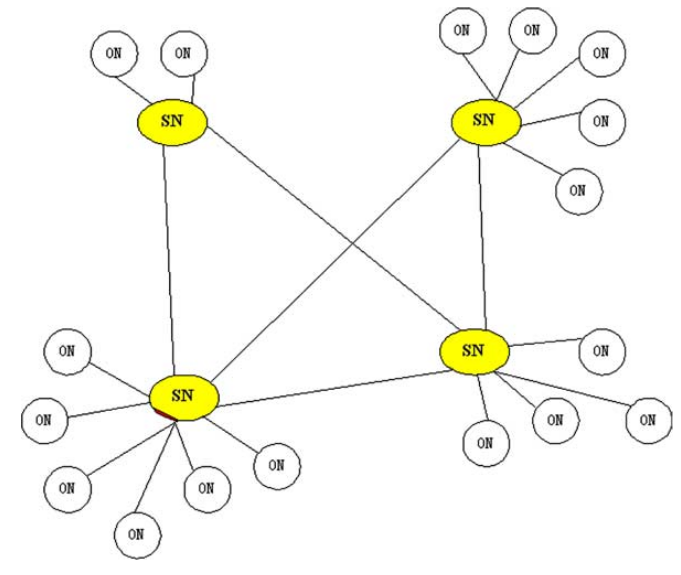
\includegraphics[scale=0.3]{gfx/aufbau}
\caption{Aufbau des FastTrack Netzwerkes (Quelle \cite{liang2006fasttrack})}
\label{fig:auf}
\end{figure}

\subsection{Knoten Programm Aufbau}
\label{subsec:proAuf}

Die offiziellen Klienten \textit{Kazaa}\cite{kazaa} sind nur für Windows vorhanden
Er besteht aus vier Komponenten, die folgend vorgestellt werden:

\begin{itemize}
\item[1.] \textbf{GUI:} Die GUI des Windows Klienten für die Eingab von Suchanfragen und anzeigen der Downloads.
\item[2.] \textbf{Windows Register:} In der Windows Registry ist der Cache der SuperKnoten gespeichert.
Dieser enthält für jeden Knoten die IP, den Port, die Auslastung und einen Zeitangabe, wann die Information das letzte mal aktualisiert wurden.
\item[3.] \textbf{DDB Dateien:} In den DDB Dateien sind die Metainformation der eigenen Dateien gespeichert. Es wird der Name, die Größe, der ContentHash und die Beschreibung der Daten. Diese werden zum Beispiel für die Suche verwendet, wenn die Metadaten zum SN gesendet werden.
\item[4.] \textbf{DAT-Dateien:} Diese Dateien enthalten die heruntergeladenen Daten, welche am Ende umbenannt werden.
\end{itemize}



\section{Funktionsweise}
\label{sec:funkw}
In diesem Abschnitt werden die bekannten Funktionsweisen und Nachrichten von FastTrack beschrieben.
Dabei werden die Informationen in allen folgenden Abschnitten aus der Studie \cite{liang2006fasttrack} von genommen.
Zuerst werden in \ref{subsec:nachricht} auf die Nachrichten, welche über FastTrack verschickt werden, beschrieben.
Danach wird im Abschnitt \ref{subsec:join} das Verbinden zum FastTrack Netzwerk dargestellt.
Es wird dann in \ref{subsec:sntosn} der Austausch von Metadaten zwischen Superknoten beschrieben.
Im Anschluss wird in \ref{subsec:search} auf die Suche im Netzwerk eingegangen.

\subsection{Nachrichten}
\label{subsec:nachricht}

Im FastTrack Netzwerk gibt es vier verschiedene Nachrichtentypen für den Austausch von Informationen. Folgende Nachrichtentypen gibt es:

\begin{itemize}
\item[1.] \textbf{Signal Nachrichten:} Diese Nachrichten dienen zum Austausch von Informationen im Netzwerk.
Zum einen um mitzuteilen, wenn sich ein Knoten das Netzwerk betreten will.
Ein Knoten Metainfomationen zum SN senden will oder ein SN aktuelle Informationen seines SN Caches mit einen normalen Knoten oder anderen SN austauschen will.
Außerdem werden darüber die Suchanfragen geschickt.
Wichtig ist, dass alle Signal Nachrichten verschlüsselt übertragen werden.
Deshalb muss am Anfang einer Übertragung ein Schlüssel ausgetauscht werden.
\item[2.] \textbf{Daten Transport Nachrichten:} Dieser Nachrichtentyp wird zum Austausch von Daten verwendet. 
Dabei werden diese Nachrichten nicht verschlüsselt übertragen.
Für die Übertragung der Rohdaten wird HTTP verwendet.
\item[3.] \textbf{Advertise Nachrichten:} Da hinter FastTrack Firmen stehen die mittels der Werbung Geld verdient, gibt es ein Nachrichtentyp um die Werbung zu übertragen.
Dies geschieht unverschlüsselt über HTTP Nachrichten.
\item[4.] \textbf{Sofort Nachrichten:} Damit es eine Möglichkeit gibt, dass sich zwei Teilnehmer des Netzwerkes unterhalten können, gibt es Sofort Nachrichten.
In diesen werden nur Text Nachrichten übertragen.
Damit die Unterhalten nicht mit gelesen werden kann, werden diese verschlüsselt übertragen.
\end{itemize} 

\subsubsection{Signal Nachrichten}
\label{subsubsec:sigN}

In der Abbildung \ref{fig:sigN} ist der Aufbau der Signalnachrichten dargestellt.
Die \textit{Packet ID} enthält die ID des Paketes um die Nachricht zu identifizieren.
Dafür wird 1 Byte verwendet.
Im \textit{Message Type} wird angegeben, ob eine Verbindung aufgebaut werden soll, Metadaten versendet oder SN-Listen ausgetauscht werden.
Es werden dafür 2 Byte verwendet.
Der \textit{Payload} enthält die Metadaten oder SN-Listen.
Die Länge des \textit{Payload} wird in der \textit{Payload Length} gespeichert
Dafür stehen in der Nachricht 2 Byte zur Verfügung.

\begin{figure}
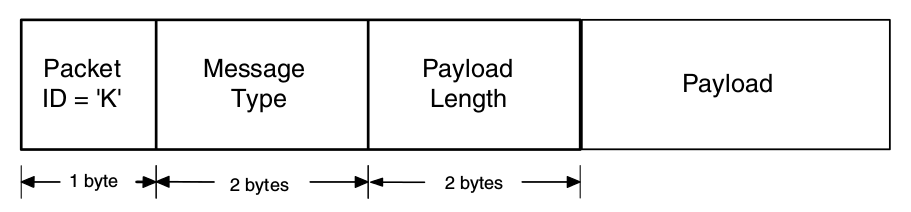
\includegraphics[scale=0.25]{gfx/signal_message}
\caption{Signal Nachricht (Quelle \cite{liang2006fasttrack})}
\label{fig:sigN}
\end{figure}

\subsection{Dem Netzwerk beitreten}
\label{subsec:join}

Der Ablauf, wenn sich ein Knoten in FastTrack Netzwerk verbindet ist in Abbildung \ref{fig:join} dargestellt.
Zuerst wählt der Knoten aus dem eigenen SN Cache ein paar SN.
Zu den gewählten SN wird eine \textit{UPD probe} Nachricht geschickt um zu testen ob der SN antworten.
Nachdem der SN geantwortet hat, wird ein TCP Handshake durchgeführt. 
Danach findet der Schlüsselaustausch statt, damit die folgenden Nachrichten verschlüsselt werden können.
Nun sendet der Knoten die Metadaten seiner Dateien zum SN.
Darunter ist auch die lokale IP, der Port und der Benutzername, des Knoten.
Mit der lokalen IP wird verhindert, dass nur der SN weiß, wo die Daten zu finden sind.
Der SN wiederum sendet eine Liste seiner bekannten SNs zum Knoten zurück.
Mit dieser Liste aktualisiert der Knoten seinen SN Cache.
Wenn der SN Cache aktualisiert ist, bricht der Knoten die Verbindung ab und sucht sich aus der aktualisierte Listen einen Eltern SN. 
Mit welchem er sich verbindet und ihm seine Metadaten und lokale Information schickt.
Die Möglichkeit der Wahl des Eltern SN wird in \ref{subsubsec:wElternSN} erläutert.
An diesem Eltern SN kann nun die Suchanfragen geschickt werden.

\begin{figure}
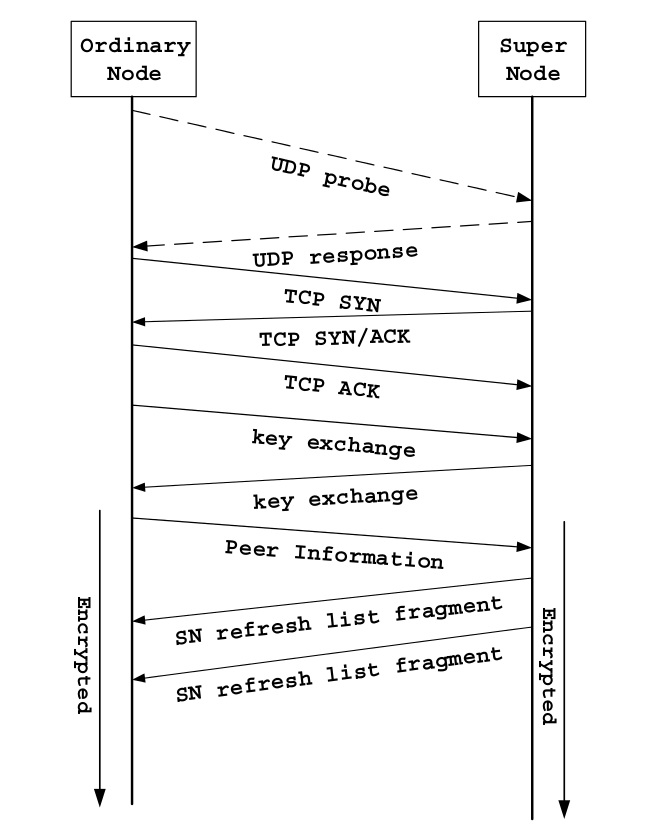
\includegraphics[scale=0.3]{gfx/join}
\caption{Nachrichten beim Verbindungsaufbau (Quelle \cite{liang2006fasttrack})}
\label{fig:join}
\end{figure}

\subsubsection{Wahl des Eltern SN}
\label{subsubsec:wElternSN}

Im Paper \cite{liang2006fasttrack} ist beschrieben, das nicht genau bekannt ist, nach welchen Kriterien der Eltern SN gewählt wird. 
Es werden zwei Möglichkeiten in Betracht gezogen.
Zum einen die Lokalität, dass heißt wie weit der SN vom Knoten entfernt ist und zum anderen die Auslastung des SN.
Bei der Lokalität wird der RoundTripTime durch einen Ping zum SN gemessen.
In der Messung \ref{fig:rtt} ist zu erkennen, dass die meisten Knoten mit SN in ihrer Nähe verbunden sind.
Ein anderer Aspekt ist die Auslastung eines SN.
Dabei spielt es eine Rolle wie viele normale Knoten ein SN schon verwaltet.
Die Information der Auslastung wird mit im SN Cache des Knoten gespeichert, welcher beim betreten des Netzwerkes aktualisiert ist.
In der Abbildung \ref{fig:workl} ist zu erkennen, dass in der Messung der Eltern SN durchschnittlich mit einer geringen Auslastung gewählt werden.
Somit sind beide Kriterien, die Lokalität sowie die Auslastung des SN, ausschlaggebend in der Wahl des Eltern SN.

\begin{figure}
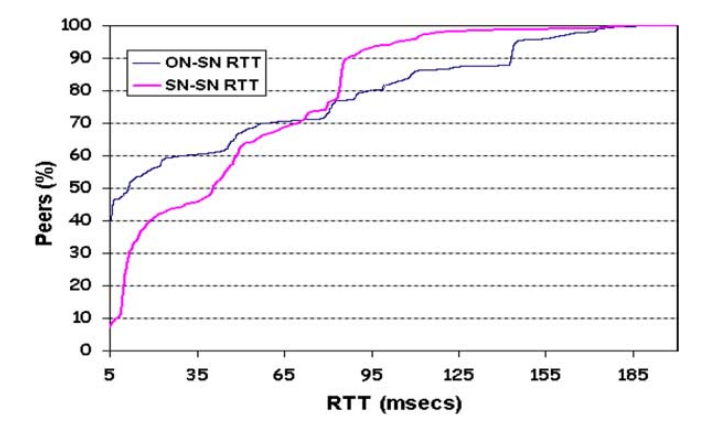
\includegraphics[scale=0.3]{gfx/rttSns}
\caption{RTT Knoten zu SN und SN zu SN (Quelle \cite{liang2006fasttrack})}
\label{fig:rtt}
\end{figure}

\begin{figure}
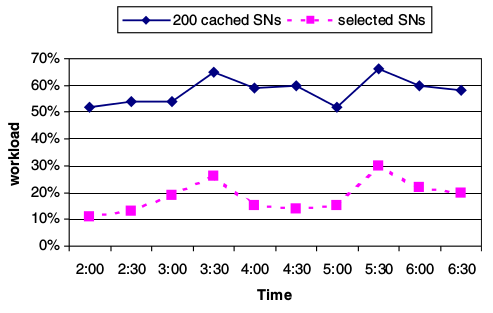
\includegraphics[scale=0.45]{gfx/workload}
\caption{Auswahl des Eltern SN nach Auslastung (Quelle \cite{liang2006fasttrack})}
\label{fig:workl}
\end{figure}

\subsection{Datenaustausch zwischen Superknoten}
\label{subsec:sntosn}

Der Ablauf wie die Superknoten untereinander ihre Daten austauschen ist in der Abbildung \ref{fig:snsn} dargestellt.
Zuerst wählt der SN einen SN aus seinem Cache.
Mit dem gewählten SN wird ein TCP Handshake durchgeführt um sich zu verbinden.
Da die Nachrichten verschlüsselt werden sollen, wird nach dem TCP Handshake ein Schlüssel ausgetauscht.
Danach senden die SN verschlüsselt ihre aktuellen bekannten SNs um ihren Cache zu aktualisieren.

\begin{figure}
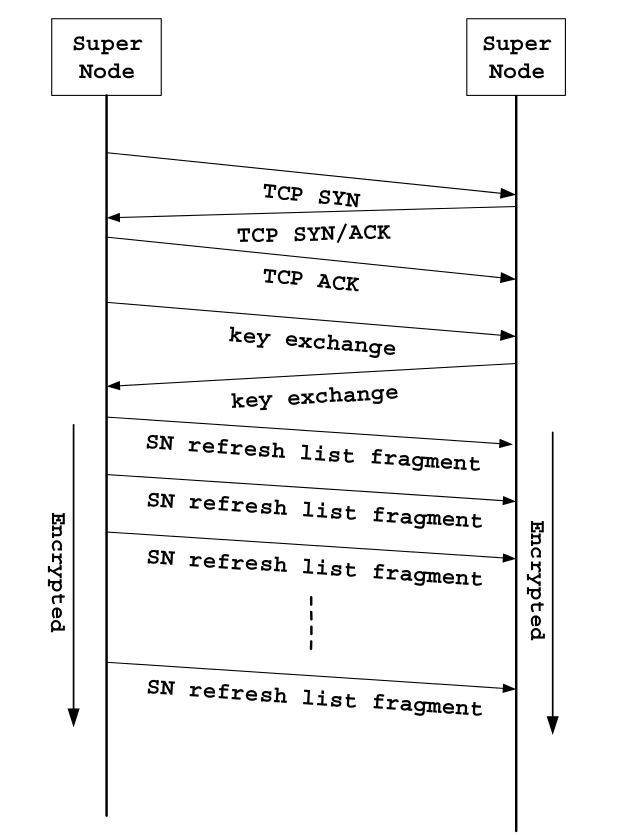
\includegraphics[scale=0.3]{gfx/SnToSn}
\caption{Nachrichten beim Austausch von Informationen zwischen SNs(Quelle \cite{liang2006fasttrack})}
\label{fig:snsn}
\end{figure}

\subsection{Suche im Netzwerk}
\label{subsec:search}

Wenn ein Knoten ein Datei suchen will, sendet dieser seinen Suchanfrage an seinen Eltern SN.
Dieser durchsucht die Metadaten seine bekannten Knoten anhand der Wörter in der Suchanfrage und schickt die Antwort ob etwas gefunden wird zurück.
Außerdem wird die Suchanfrage an seine bekannte SN gesendet, damit dieser in den Metadaten seiner bekannten Knoten.
Mit der Antwort, kann der Knoten nun den Download starten.
In Sektion \ref{subsubsec:dnat} wird beschrieben wie der Download stattfindet, wenn der Knoten, welcher die Datei besitzt hinter eine Nat sitzt.

\subsubsection{Download über NAT}
\label{subsubsec:dnat}
Da es häufig vorkommt, dass die Knoten B hinter einem NAT sitzen, gibt es die Möglichkeit über den Eltern SN des jeweiligen Knoten, den Download zu starten.
Wenn ein Knoten A einen Download starten will, dann hat er die IP Adresse des Knoten B, daran erkennt er ob es eine lokale oder globale Adresse handelt.
Bei einer lokalen Adresse fragt er den Eltern SN des Knoten B, dass er von Knoten B eine Datei herunterladen will und nur die lokale Adresse kennt.
Der Eltern SN von B, teilt nun Knoten B mit, das Knoten A eine Datei von ihm herunterladen will.
Diese Nachricht enthält die globale Adresse von A.
Nun verbindet sich Knoten B mit Knoten A und Knoten A kann die Datei von B herunterladen.

\section{Probleme und Weiterführende Informationen}
\label{sec:last}
In diesem Abschnitt geht es darum auf die Probleme \ref{subsec:probT} von FastTrack einzugehen.
Außerdem wird im letzten Teil \ref{subsec:impl} angegeben, welche Implementierung es vom FastTrack Protokoll gibt und ein kurzer Überblick wie es damit weiter ging.


\subsection{Probleme von FastTrack}
\label{subsec:probT}

Eines der Probleme, welche aus dem Messungen von \cite{liang2006fasttrack}, wie in Abbildung \ref{fig:rtt} zu erkennen ist, dass die Round Trip Time von etwa 85 \% der SN zu SN Verbindungen bei maximal 100 ms beträgt.
Wie in der Abbildung \ref{fig:rttcaida} von Caida.org von 2001 \cite{caida} zu erkennen, beträgt die Round Trip Time von Amerika nach Europa und Asien etwa 200 ms.
Somit wird es schwierig das ganze Netzwerk zu durchsuchen, da nur wenige der SN über Verbindungen verfügen, welche weiter entfernt sind.

\begin{figure}
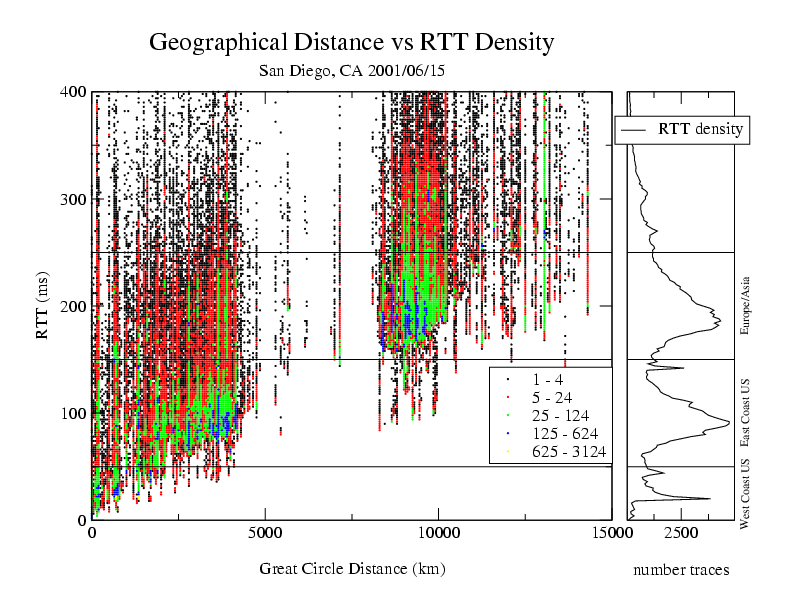
\includegraphics[scale=0.3]{gfx/dist_density_rie_20010513}
\caption{RTT Messung von Caida (Quelle \cite{caida})}
\label{fig:rttcaida}
\end{figure}


\subsubsection{UHASH}
\label{subsubsec:uhash}

Ein weiteres Problem ist der Content Hash Funktion UUHash \cite{uuHash} von FastTrack.
Der Hash kann schnell berechnet werden, da nur alle $2^n, n \in \mathbb{N}$ die ersten 300 KiB in die Berechnung einfließen.
Somit ist es möglich die Bereiche, welche nicht zur Hash Berechnung verwendet wurde mit Schadcode zu einzufügen.
Dies führte jedoch auch zu einem Problem, so das 2005 etwa 50\% aller Dateien infiziert waren. \cite{menneck2} 
Da viele MP3s über FastTrack getauscht werden und die Musikfirmen dies verhindern wollen, wurden viele MP3s kompromittiert um die Anwender zu schädigen. \cite{veitinger2002}


\subsection{Implementationen}
\label{subsec:impl}

Die offizielle Implementierung des FastTrack Netzwerkes ist Kazaa \cite{kazaa} von den Beiden FastTrack Entwicklern.

Eine verbreitete inoffizielle Implementierung ist die Kazaa-Lite \cite{kazaaLite} Version.
Diese verwendet bei der Suche nicht nur den Eltern SN sondern versucht an mehrere SNs seine Suchanfrage zu senden.
Dabei wird zuerst die Anfrage an den Eltern SN gesendet und auf die Antwort gewartet.
Wenn der Knoten die Antwort erhält schließt dieser die Verbindung und sendet die Anfrage an einen neuen SN.\cite{liang2006fasttrack}

Zwei andere Implementierungen, welche das FastTrack Netwerk benutzten sind Grokster \cite{grokster} und Morpheus \cite{morpheus}, wobei Morpheus 2002 auf das Gnutella \cite{gnutella} Netzwerk umgestiegen ist. \cite{morphvsKazaa}

Außerdem gibt es eine Implementierung für giFT \cite{gift}, dies ist eine Sammlung für Peer-To-Peer Protokolle und FastTrack wurde per reverse Engineering als Plugin hinzugefügt \cite{liang2006fasttrack}

Eine der bekanntesten Weiterentwicklung die auf FastTrack basiert und aufbaut ist Skype \cite{skypeAna}, welches von den selben Entwicklern entwickelt wurde.
\bibliography{bibliography}
\end{document}
